\subsection{rpc.go}

The data structures defined here are: \emph{id}, \emph{header}, \emph{Call}, \emph{callId}, \emph{Server} and \emph{Client}. The most important are \emph{Server} and \emph{Client}.\\
Type Server contains a \emph{reflect.Value} used during the creation of the Server, an array of \emph{int} which contains the indexes of the exported methods the Server is supposed to respond to, an \emph{Encoder} and a \emph{Decoder}, used to transmit and receive values.\\
Type Client contains a map where the element type is \emph{*Call} and the key type is \emph{int} to keep track of the calls, an \emph{Encoder} and a \emph{Decoder}.
Type Call contains two interfaces (one for the arguments and the other for the reply), an \emph{os.Error} and a boolean \emph{Channel}.\\
Here the constructors of \emph{Server} and \emph{Client}:

\begin{itemize}
 
\item \emph{func NewServer(v interface{}, e *Encoder, d *Decoder) (s *Server)}\\
It creates a server using the value stored in the empty interface that transmits and receives values using the supplied Encoder and Decoder. The newly-created server will respond to the exported methods of this value.

\item \emph{func NewClient(e *Encoder, d *Decoder) *Client}\\
It creates a client that transmits and receives values using the supplied Encoder and Decoder.

\end{itemize}
Here the function of \emph{callId} type:

\begin{itemize}

\item \emph{func (c *callId) Increment() (i id)}\\
It locks variable c, increments its id, unlocks c and returns the \emph{c} previous id.  

\end{itemize}
Here the functions of \emph{Client} type:

\begin{itemize}

\item \emph{func (c *Client) Dispatch() bool}\\
It collects, decodes and dispatches replies.

\item \emph{func (c *Client) Go(id uint64, args, reply interface{}) (call *Call)}\\
It creates a new call using the parameters. If either \emph{call.reply} or \emph{c.d} (Client's decoder) are \emph]{nil}, the call is done, otherwise, the call is added to the Client's calls map.

\item \emph{func (c *Client) Call(id uint64, args, reply interface{}) (err os.Error)}\\
Synchronous function. It uses method \emph{Go} to create a new call and does not return until call is finished. 

\end{itemize}
Here the function of \emph{Server} type:

\begin{itemize}

\item \emph{func (s *Server) Handle() os.Error}\\
It handles \emph{Server}'s requests.

\end{itemize}


\begin{figure}[H]
\centering
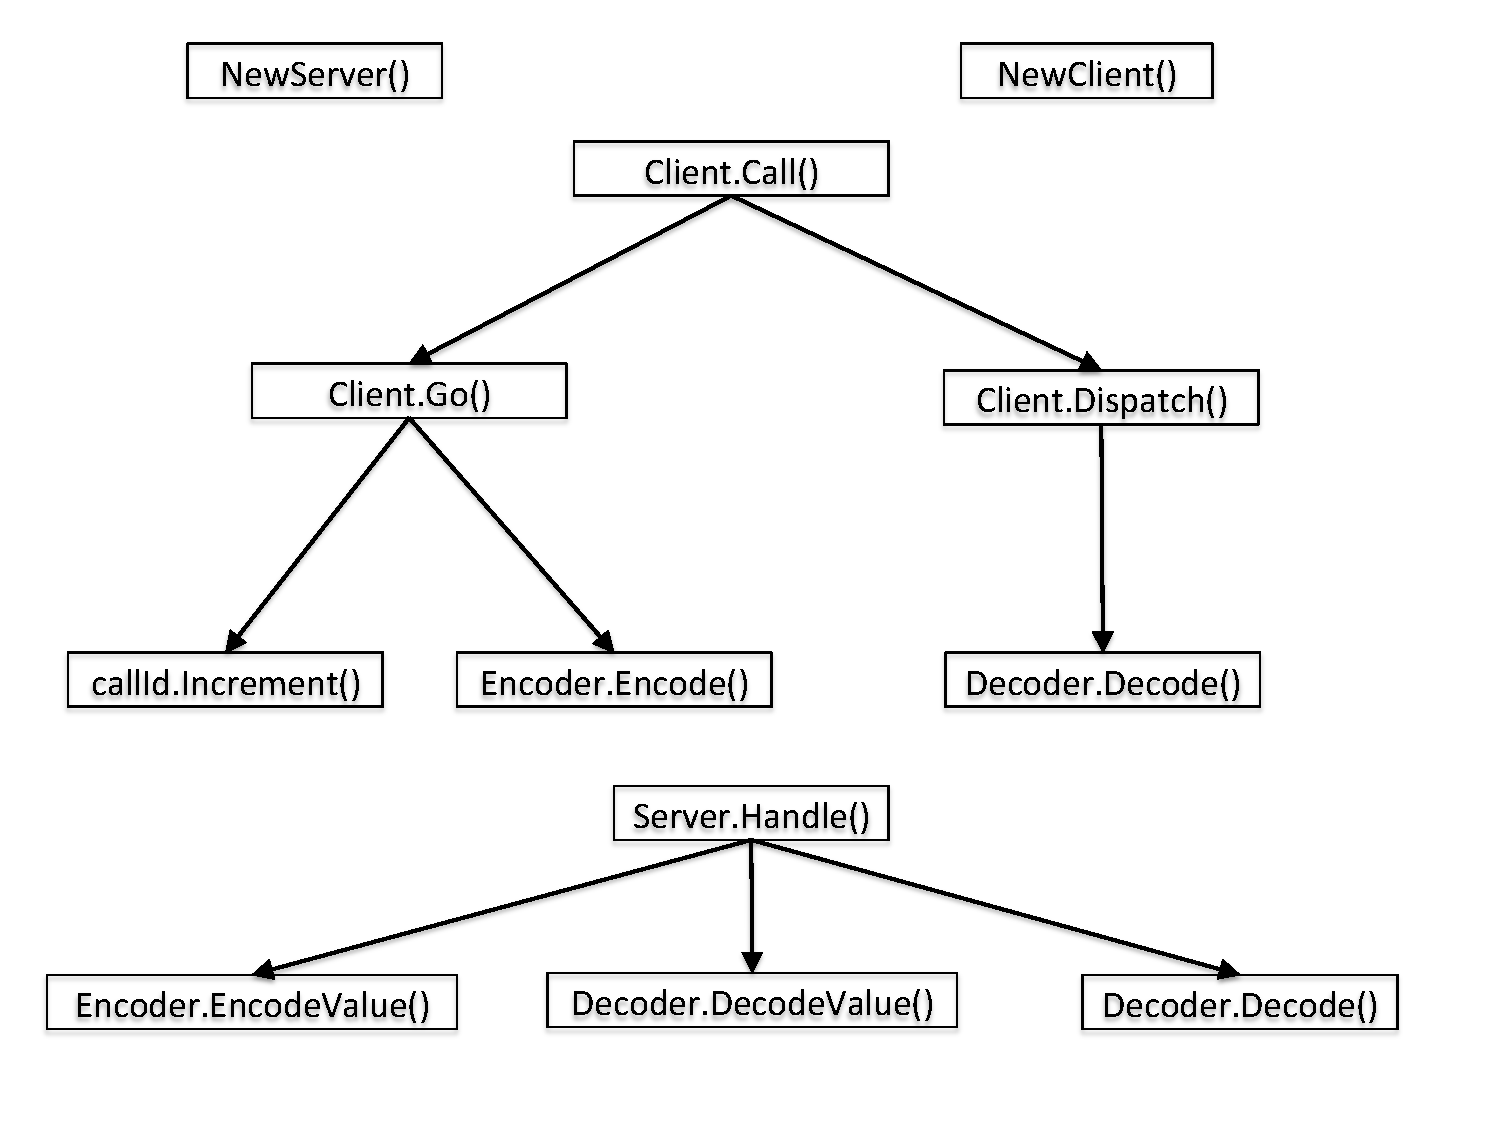
\includegraphics[scale=0.50]{rpcPackage}
\caption{rpc.go package}
\end{figure}